%FOR PDFLATEX USE ONLY
\documentclass[a4paper,12pt]{article}

\usepackage{amssymb,amsmath} %math symbols

\usepackage[margin=2cm]{geometry} %paper geometry

\usepackage[utf8]{inputenc} %allows unicode (including russian) source file
\usepackage[russian]{babel} %docment in russian-style
\usepackage[utf8]{inputenc}
\usepackage[unicode]{hyperref} %links inside of the text
\usepackage[pdftex]{graphicx} %includegraphics pictures
\usepackage{cmlgc} %bold text

\usepackage{array} %arrays

\usepackage{wrapfig}
\usepackage{array}
\usepackage{lipsum}
\usepackage{esvect}
\usepackage{hyperref}

\usepackage{subfig}
\usepackage{calc}
\usepackage{pgfplots,tikz,circuitikz}
\usepackage{tkz-euclide}

\usepackage{import}
\usepackage{xifthen}
\usepackage{pdfpages}
\usepackage{transparent}

\newcommand{\incfig}[1]{%
    \def\svgwidth{\columnwidth}
    \import{./figures/}{#1.pdf_tex}
}

\begin{document}
\begin{center}
  \LARGE{Работа 1.2.5}\\[0.2cm]
  \LARGE{Исследование прецессии уравновешенного гироскопа}\\[0.2cm]
  \large{Малиновский Владимир}\\[0.2cm]
  \normalsize{\texttt{galqiwi@galqiwi.ru}}
\end{center}

\textbf{Цель работы:} исследовать вынужденную прецессию гироскопа, установить зависимость скорости вынужденной прецессии от величины момента сил, действующий на ось гироскопа и сравнить ее со скоростью, рассчитанной по скорости прецессии.
\textbf{В работе используются:} гироскоп в кардановом подвесе, секундомер, набор грузов, отдельный ротор гироскопа, цилиндр известной массы, крутильный маятник, штангенсциркуль, линейка.

\section*{Теория}

В этой работе исследуется зависимость скорости прецессии гироскопа от момента силы, приложенной к его оси. Для этого к оси гироскопа подвешиваются грузы. Скорость прецессии определяется по числу оборотов рычага воеруг вертикальной оси и времни, которое на это ушло, определяемоу секундомером. В процессе измерений рычаг не только поворачивается в результате прецессии гироскопа, но и опускается. Поэтому его в начале опыта следует преподнять на 5-6 градусов.  Опять надо закончить, когда рычаг опустится на такой же угол.\\
\begin{center}$
\begin{array}{cc}
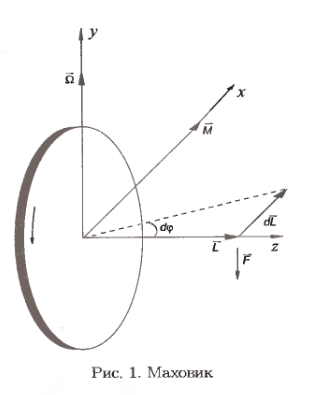
\includegraphics[width=0.40\textwidth]{img1.png}&
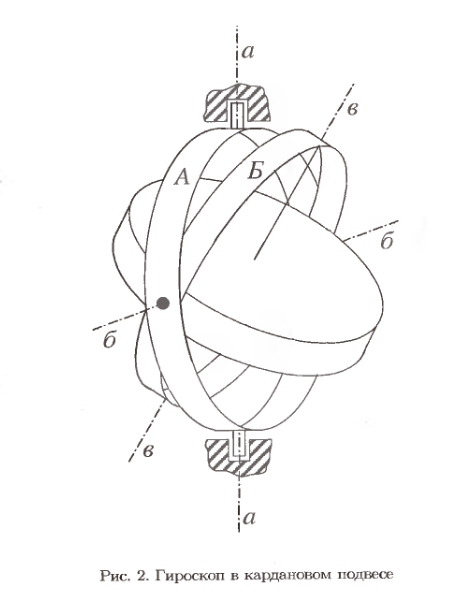
\includegraphics[width=0.40\textwidth]{img2.png}\\
\end{array}$
\end{center}
Измерение скорости прецессии гироскопа позволяет вычислить угловую скорость вращения его ротора. Расчет производится по формуле:
\begin{equation}
	\Omega = \frac{mgl}{I_z\omega_0},
\end{equation}
где $m$ -- масса груза, $l$ -- расстояние от центра карданова подвеса до точки крепления груза на оси гироскопа, $I_z$ -- момент инерции гироскопа по его главной оси вращения. $\omega_0$ -- частота его вращения относительно главной оси, $\Omega$ -- частота прецессии.\\
Момент инерции ротора относительно оси симметрии $I_0$ измеряется по крутильным колебаниям точной копии ротора, подвешиваемой вдоль оси симметрии на десткой проволоке. Период крутильных колебаний $T_0$ зависит от момента инерции $I_0$ и модуля кручения проволоки $f$:
\begin{equation}
	T_0 = 2\pi\sqrt{\frac{I_0}{f}}.
\end{equation}
Чтобы исключить модуль кручения проволоки, вместо ротора гироскопа к той же проволоке подвешивают цилиндр правильной формы с известными размерами и массой, для которого легко можно вычислить момент инерции $I_\text{ц}$. Для определения момента инерции ротора гироскопа имеем
\begin{equation}
	I_0 = I_\text{ц}\frac{T_0^2}{T_\text{ц}^2},
\end{equation}
Здесь $T_\text{ц}$ -- период крутильных колебаний цилиндра.\\
\begin{center}
	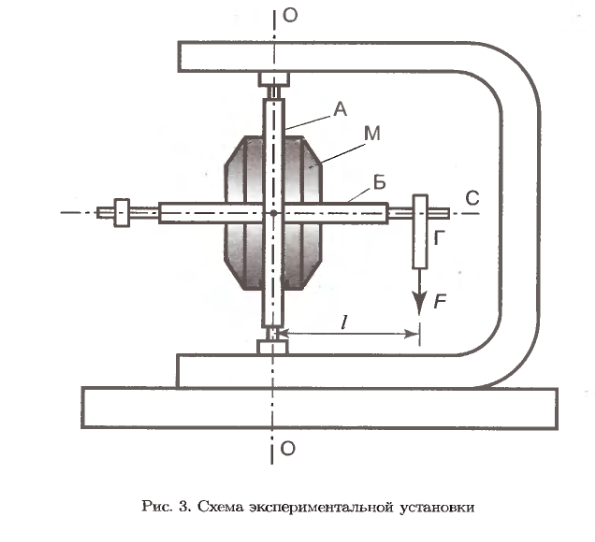
\includegraphics[width=0.8\textwidth]{img3.png}
\end{center}
Скорость вращения ротора гироскопа можно определить и не прибегая к исследованию прецессии. У используемых в работе гироскопов статор имеет две обмотки, необходимые для быстрой раскрутки гироскопа. В данной работе одну обмотку искользубт для раскрутки гироскопа, а вторую -- для измерения числа оборотов ротора. Ротор электромотора всегда немного намагничен. Вращаясь, он наводит во второй обмотке переменную ЭДС индукции, частота которой равна частоте врещения ротора. Частоту этой ЭДС можно, в частности, измерить по фигурам Лиссажу, получаемым на экране осциллографа, если на один вход подать исследуемую ЭДС, а на другой -- переменное напряжение с хорошо прокалиброванного генератора. При совпадении частот на эеране получаем эллипс.

\section*{Результаты и обработка}
Данные для частоты прецессии и опускания гироскопа:
\begin{center}
\begin{tabular}{|c|c|c|c|c|c|c|c|}
\hline
$m, \text{г}$ & $t, \text{с}$ & $h_0, \text{мм}$ & $h_1, \text{мм}$ & $a_0, ^\circ$ & $a_1, ^\circ$ & $\Omega, 10^{-3}\text{с}^{-1}$ & $\Omega_f, 10^{-3}\text{с}^{-1}$\\
\hline
$57$ & $75.5$ & $155$ & $136$ & $210$ & $336$ & $29.1\pm 0.6$ & $2.0\pm 0.2$ \\
\hline
$76$ & $77.3$ & $155$ & $132$ & $358$ & $532$ & $39.3\pm 0.7$ & $2.4\pm 0.2$ \\
\hline
$91$ & $77.6$ & $155$ & $132$ & $220$ & $430$ & $47.2\pm 0.7$ & $2.4\pm 0.2$ \\
\hline
$93$ & $75.8$ & $155$ & $136$ & $42$ & $250$ & $47.9\pm 0.7$ & $2.0\pm 0.2$ \\
\hline
$116$ & $76.8$ & $155$ & $133$ & $248$ & $512$ & $60.0\pm 0.8$ & $2.3\pm 0.2$ \\
\hline
$141$ & $80.2$ & $155$ & $133$ & $198$ & $538$ & $74.0\pm 0.8$ & $2.2\pm 0.2$ \\
\hline
$215$ & $75.7$ & $155$ & $134$ & $168$ & $658$ & $113.0\pm 1.1$ & $2.2\pm 0.2$ \\
\hline
$267$ & $85.8$ & $155$ & $130$ & $228$ & $916$ & $140.0\pm 1.1$ & $2.3\pm 0.2$ \\
\hline
$335$ & $71.5$ & $155$ & $132$ & $226$ & $948$ & $176.2\pm 1.5$ & $2.6\pm 0.2$ \\
\hline
\end{tabular}
\end{center}
Где $m$ -- масса груза, $t$ -- время измерения, $h_0$, $h_1$ -- высоты края гироскопа до и после измерения соответственно, $a_0$, $a_1$ -- углы поворота гироскопа в горизонтальной плоскости до и после измерения соответственно. $\Omega$, $\Omega_f$ -- угловые скорости прецессии и опускания гироскопа, рассчитанные по формулам:
\begin{equation}
	\Omega = \frac{a_1 - a_0}{t},
\end{equation}

\begin{equation}
	\Omega_f = \frac{asin((h_0 - h_z) / L) - asin((h_1 - h_z) / L)}{t},
\end{equation}

где $h_z$ -- высота края гироскопа в горизонтальном положении, равная $145\pm 0.5 \text{мм}$, а $L$ -- расстояние от центра до края, равное $126.2\pm 0.7 \text{мм}$.

Погрешности измерений равны: $\Delta t = 0.4 \text{с}$, $\Delta h = 0.5 \text{мм}$, $\Delta a = 1^\circ$. 

Поскольку момент сил трения не зависит от нагрузки $m$, угловая скорость опускания гироскопа так же не зависит от $m$, что видно из данных в таблице выше. Среднее значение $\Omega_f$ равно:
\begin{equation}
	< \Omega_f> = (2.3\pm 0.2)\cdot10^{-3}\text{с}^{-1}
\end{equation}

\newpage
Из формулы (1) видна линейность скорости прецессии и массы, рассмотрим эту зависимость на эспериментальных данных:
\begin{center}
	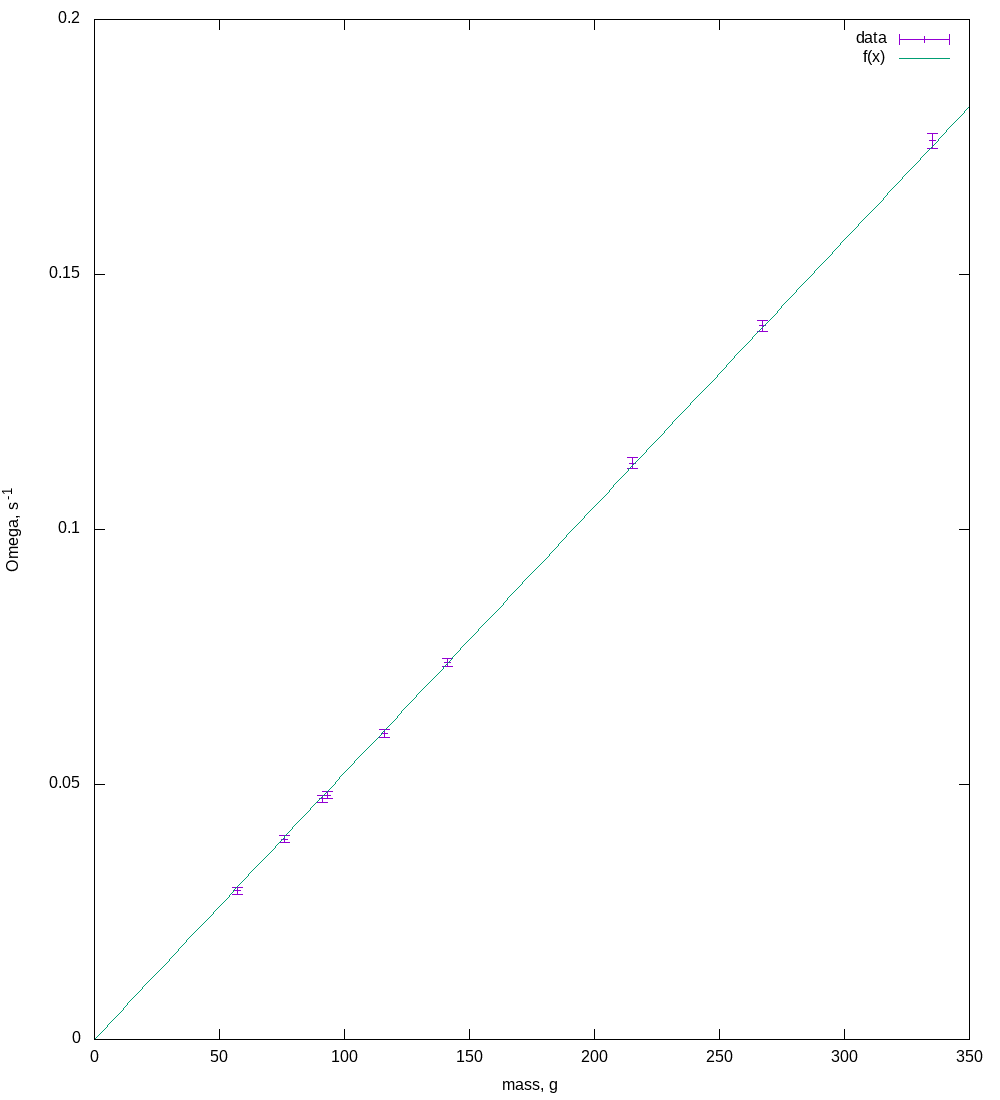
\includegraphics[width=0.95\textwidth]{plot0.png}
\end{center}

Из МНК следует, что коэффициент пропорциональности равен:
\begin{equation}
	\frac{gl}{I_z\omega_0} = (0.5225 \pm 0.0015) \frac{1}{\text{с} \cdot \text{кг}}.
\end{equation}

Измерение момента инерции.

Параметры калибровочного цилиндра (Масса и диаметр соответственно):
\begin{equation}
	M = (1617.4\pm 0.1) \text{г}, D = (78.2 \pm 0.1) \text{мм}.
\end{equation}
Периоды вращения цилиндра и гироскопа:
\begin{center}
\begin{tabular}{|c|c|c|c|c|c|c|}
\hline
& $T_{10}, \text{с}$ & $T_{10}, \text{с}$ & $T_{10}, \text{с}$ & $T_{10}, \text{с}$ & $T_{10}, \text{с}$ & <T>, \text{c} \\
\hline
\text{гироскоп} & $32.41$ & $32.53$ & $32.39$ & $32.66$ & $32.59$ & $3.25\pm 0.04$\\
\hline
\text{цилиндр} & $40.94$ & $41.05$ & $40.90$ & $41.04$ & $40.96$ & $4.10\pm 0.04$\\
\hline
\end{tabular}
\end{center}

Из этого рассчетный момент инерции гироскопа равен:
\begin{equation}
	I_z = \frac{M D^2}{8} \left( \frac{T_g}{T_\text{ц}} \right)^2 = (7.8\pm 0.4) \cdot 10^{-4} \;\; \text{кг} \cdot \text{м}^2.
\end{equation}

Из (7) и (9) получаем частоту вращения гироскопа ($l = 121\text{мм}$):
\begin{equation}
\omega_0 = (2.91 \pm 0.16) \cdot 10^{3}\;\; \text{с}^{-1},
\end{equation}

\begin{equation}
f_0 = (463\pm 25) \text{с}^{-1}.
\end{equation}

Измерение момента сил трения:

\begin{equation}
	M_f = I_z \omega_0 \Omega_f = (5.223\pm 0.015)\;\; \text{мН} \cdot \text{м}.
\end{equation}

Нахождение частоты вращения гироскопа по затуханию:

\begin{center}
\begin{tabular}{|c|c|c|c|c|c|c|c|c|c|c|}
\hline
$t, \text{с}$ & $69.9$ & $124.7$ & $152.9$ & $181.1$ & $210.2$ & $240.3$ & $270.1$ & $300.0$ & $330.8$ & $362.6$ \\
\hline
$f, \text{Гц}$ & $440$ & $420$ & $410$ & $400$ & $390$ & $380$ & $370$ & $360$ & $350$ & $340$ \\
\hline
\end{tabular}
\end{center}
\begin{center}
\begin{tabular}{|c|c|c|c|c|c|c|c|c|c|c|}
\hline
$t, \text{с}$ & $394.3$ & $427.8$ & $462.0$ & $496.4$ & $532.2$ & $568.9$ & $607.6$ & $646.5$ & $686.5$ & $725.6$ \\
\hline
$f, \text{Гц}$ & $330$ & $320$ & $310$ & $300$ & $290$ & $280$ & $270$ & $260$ & $250$ & $240$\\
\hline
\end{tabular}\\[0.2cm]
$\Delta t = 0.4 \text{с}.$
\end{center}
\begin{center}
	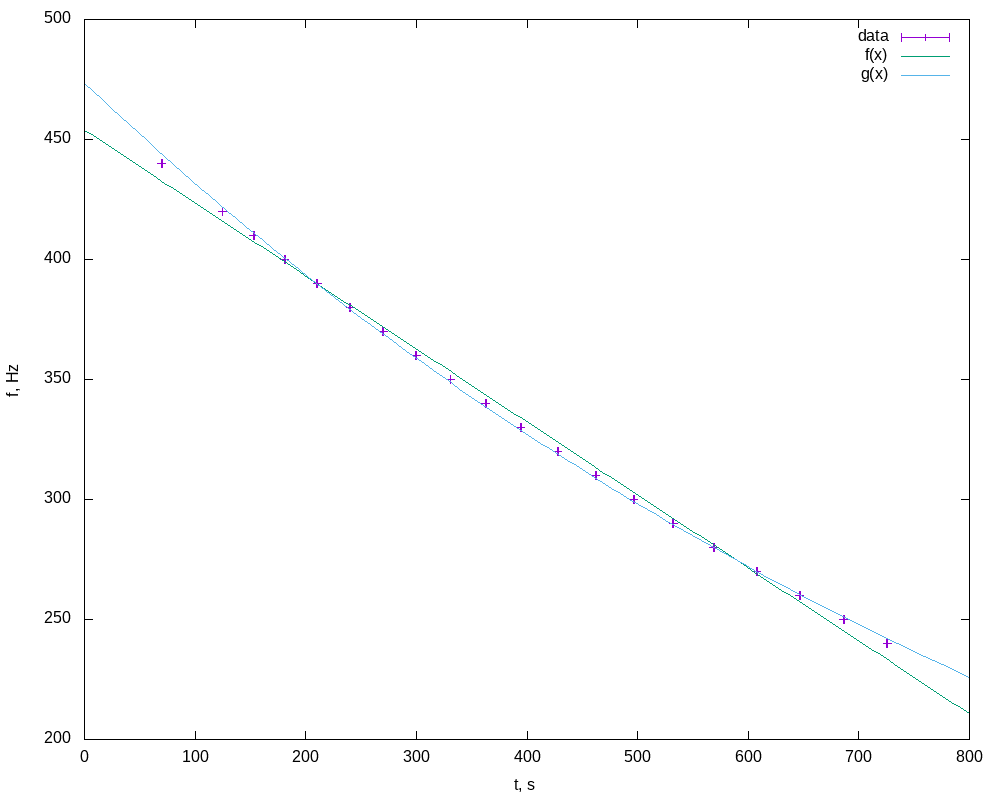
\includegraphics[width=0.95\textwidth]{f.png}
\end{center}

В линейном приближении получается частота $f_l = (454\pm 2) \text{Гц}$.\\
В экспоненциальном приближении получается частота $f_e = (473\pm 1) \text{Гц}$.\\
\newpage
Вывод:\\
В этой работе была найдена скорость вращения 3 способами -- по прецессии, и по раздичным линеаризациям затухания вращения гироскопа и момент сил трения в оси гироскопа. Различные линеаризации все находятся в погрешности измерения по прецессии, но как основную линеаризацию я бы выбрал экспоненциальное затухание -- оно лучше кладется на точки.

\end{document}